\chapter{Project Implementation} 

\section{Technology choices}

\paragraph{}
When we	started	the	project,	we	aimed	to	design	a	health	bot	running	on	the	web.	When	we	started	designing	the	healthcare	bot,	we	preferred	the	Python	programming	language	in	 terms	of	resource	abundance	and	high	implementation	speed.	In	this	context,	we	decided	to	use	Django,	the	python	web	framework.	Django	is	specialized	to	make	it	easier	to	build	web	applications	with	complex	databases\cite{bib:misc:7}.	Django	is	designed	to	have	the	principles	of	reusability, modularity,	and	rapid	development	process.	For	Chatbot,	we	used	ChatterBot,	which	is	also	a	library	of	Python	language.	ChatterBot	is	designed	for	the	development	of	bots	that	can	communicate	with	the	user	through	an	educatable	automated	dialogue\cite{bib:misc:8}.	Finally,	we	used	Scikit-Learn,	a	python	machine	learning	package,	to	get	the	symptoms	out	of	the	input.	
\paragraph{}
Due	to	the	lack	of	available	data,	we	had	to	decide	late	on	the	database	architecture.	Due	to	this	reason,	we	delayed	the	construction	of	the	application	with	django,	which	is	based	on	modeling	in	the	database.	At	the	same	time,	the	deficiencies	in	ChatterBot	and	django	integration	and	the	size	of	the	solution	learning	curve	pushed	us	to	change	technology.	For	this	reason,	we	decided	to	develop	a	Telegram	bot	as	a	tool	that	we	can	focus	only	on	bot	training\cite{bib:misc:9}.	Telegram	is	an	open	source	instant	messaging	application.	

\paragraph{}
In order to create the classifier we decided to use \textit{SciKit-learn}\cite{bib:misc:2} a python module easy to use and with wide customization possibilities. To test and visualize the results of the classifier two other tools were used : \textit{Jupyter}\cite{bib:misc:3} and \textit{matplotlib}\footnote{A python library to display plots}

\paragraph{}
The database technology that we decided to use is \textit{PostgreSQL}\cite{bib:misc:1}.
\paragraph{}
The software is open-source, which means that the source code is available at no charge. In that way if we have a need to customize or extend PostgreSQL in any way then we are able to do so with no attached costs.
\paragraph{}
PostgreSQL is available for almost every version of Unix (34 platforms with the latest stable release), and Windows compatibility is available via the Cygwin framework.
\paragraph{}
And last but not least, the legendary reliability and stability of PostgreSQL.

\section{Natural Language Recognition}

\subsection{Classifier implementation}

\paragraph{}
In	order	to	process	the	symptom	from	the	user	as	a	meaningful	message	text,	we	treat	each	symptom	stored	in	our	database	as	a	class.	In	this	way,	we	can	see	if	the	input	from	the	user	is	a	symptom	and	if	it	is	a	symptom	which	symptom	it	is.	We	created	some	training	data	for	each	symptom.	At	this	point,	we	can	catch	the	same	complaint	being	expressed	in	different	words.	For	example,	when	a	user	says	"I	have	pain	in	my	head"	instead	of	"I	have	a	headache",	we	have	a	chance	to	catch	that	the	symptom	is	actually	a	headache.	

\paragraph{}
In order to understand the symptom the user enters in as an input, a classifier is used. The dataset is composed of the symptoms and different expressions of them, per example the pair \texttt{headache : my head hurts}.

\paragraph{}
First of all, as the classes are known, a supervised method is to be used. In natural language processing the Support Vector Machine (SVM)\cite{bib:misc:6} is well known for its efficiency on supervised problems. So it has been decided to use this method. 

\begin{figure}[H]
	\centering
	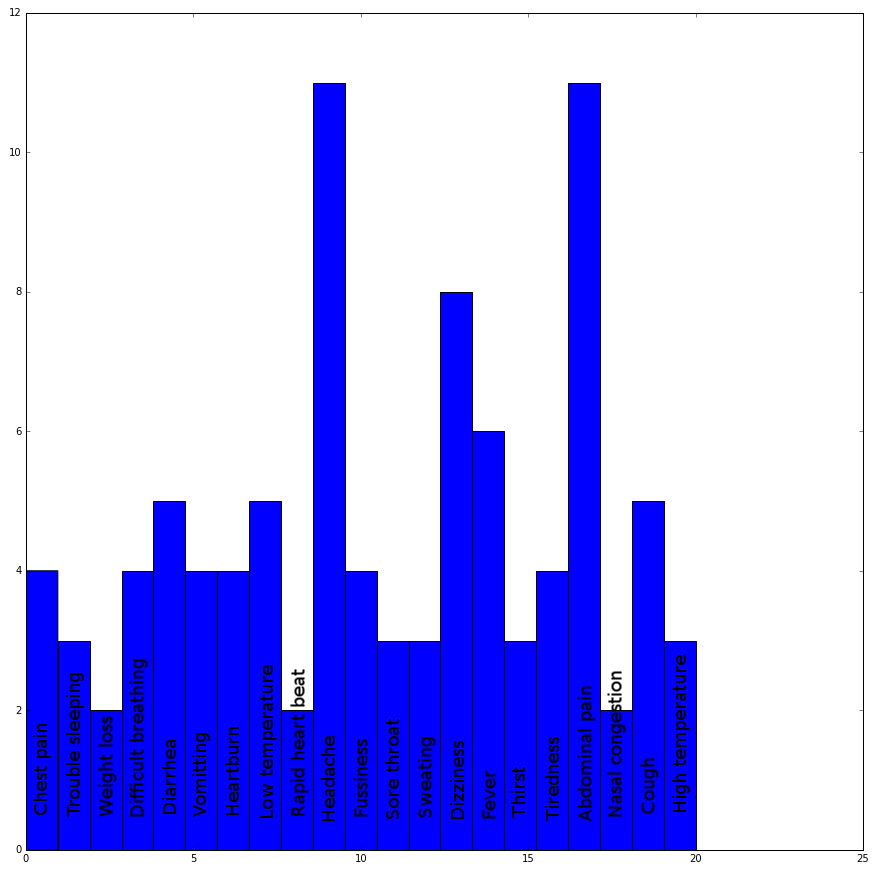
\includegraphics[height=10cm]{classifier_classes_repartition}
	\caption{Data repartition of the dataset}
	\label{dataset}
\end{figure}

\paragraph{}
Different tests has been done to obtain a good classifier. Two different implementations of SVM has been used. First the \texttt{multi-class one-against-one classification}\footnote{If $n_class$ is the number of classes, then $n_class * (n_class - 1) / 2$ classifiers are constructed and each one trains data from two classes.} with different \texttt{aggregation shapes}\footnote{To provide a consistent interface with other classifiers, the results of the “one-against-one” classifiers can be aggregate using different decision function of shape} then the \texttt{multi-class one-vs-the-rest classification}\footnote{If $n_class$ is the number of classes, then $n_class$ classifiers are constructed. If there are only two classes, only one model is trained} with a linear kernel\cite{bib:misc:5}. The main difference is that solving the optimization problem for a linear kernel is much faster than for non-linear with a negligible loss of predictive performance\cite{bib:article:1}.

\paragraph{}
In order to compare the different classifier created, we used confusion matrix. First the classifiers has been tested on the training data then the best one on a test set\footnote{Containing values that are not in the training set}. 
\newpage
\begin{multicols}{2}
	\begin{figure}[H]
		\centering
		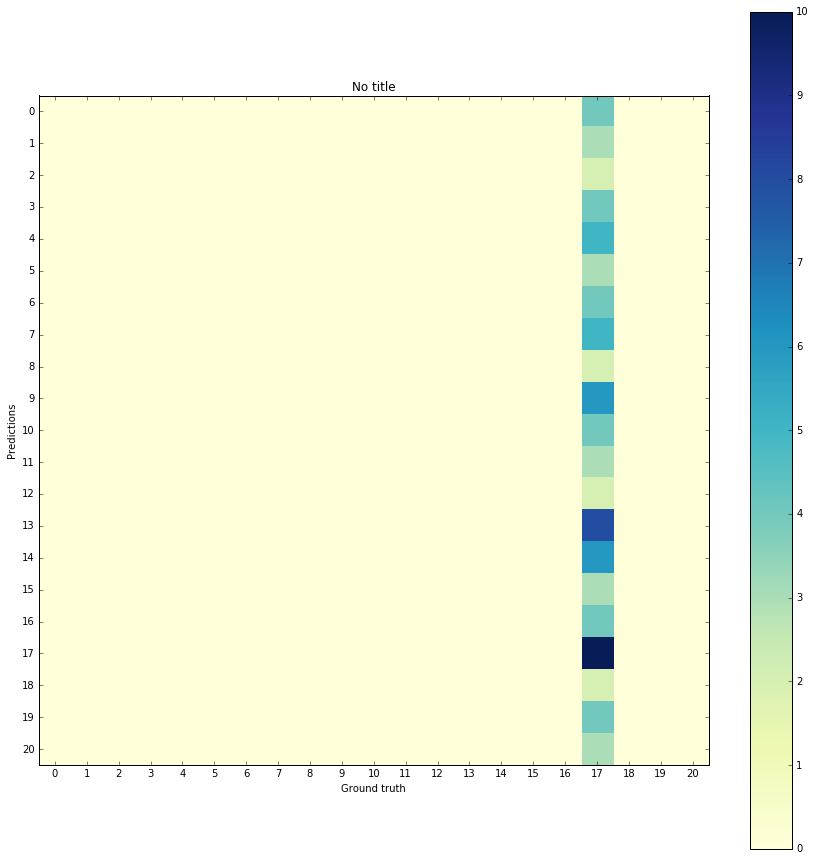
\includegraphics[width=0.4\textwidth]{classifier_svm}
		\caption{Confusion matrix for SVM}
		\label{svm}
	\end{figure}

	\begin{figure}[H]
		\centering
		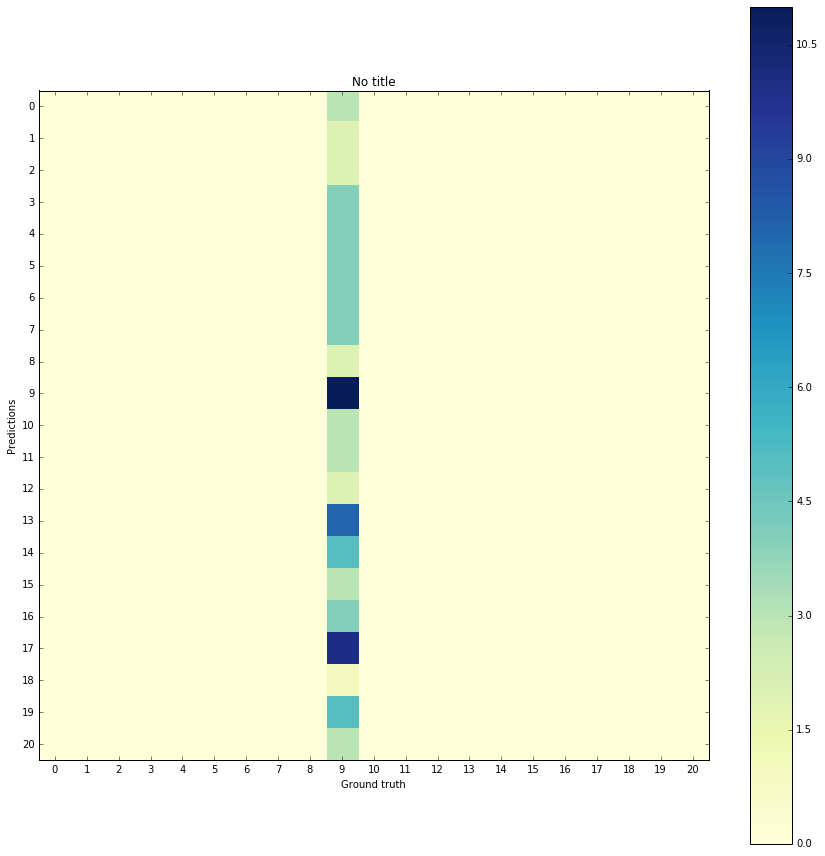
\includegraphics[width=0.4\textwidth]{classifier_svm_ovo}
		\caption{Confusion matrix for SVM using ovo aggregation function}
		\label{svm_ovo}
	\end{figure}
	
\end{multicols}

\begin{multicols}{2}
\begin{figure}[H]
	\centering
	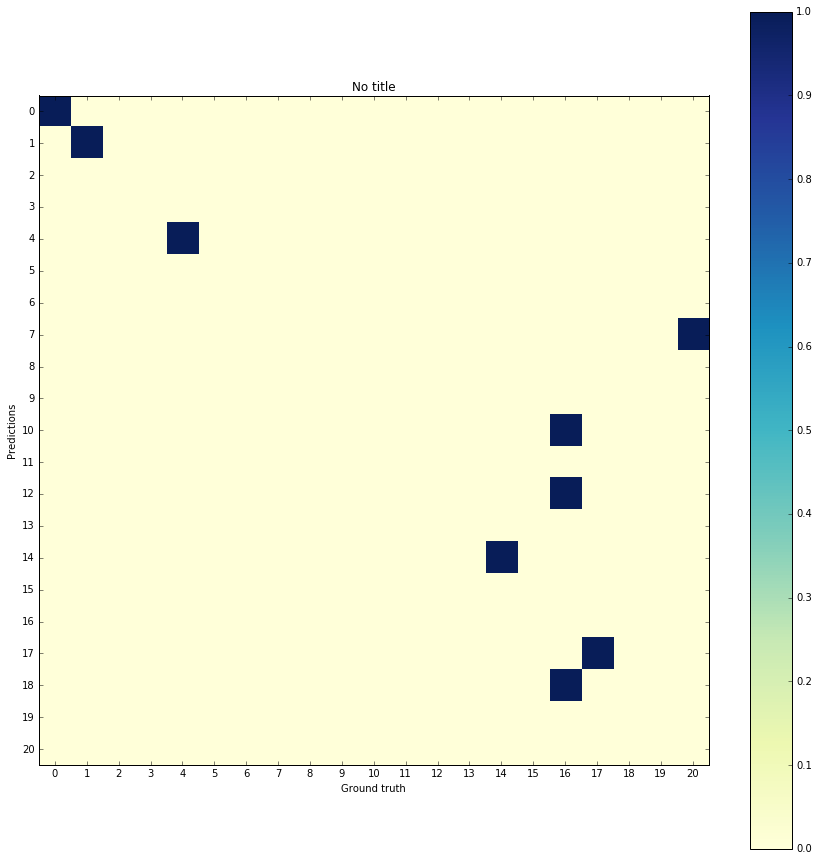
\includegraphics[width=0.4\textwidth]{classifier_svm_linear_test}
	\caption{Confusion matrix for linear SVM on test set data}
	\label{svm_test}
\end{figure}

\begin{figure}[H]
	\centering
	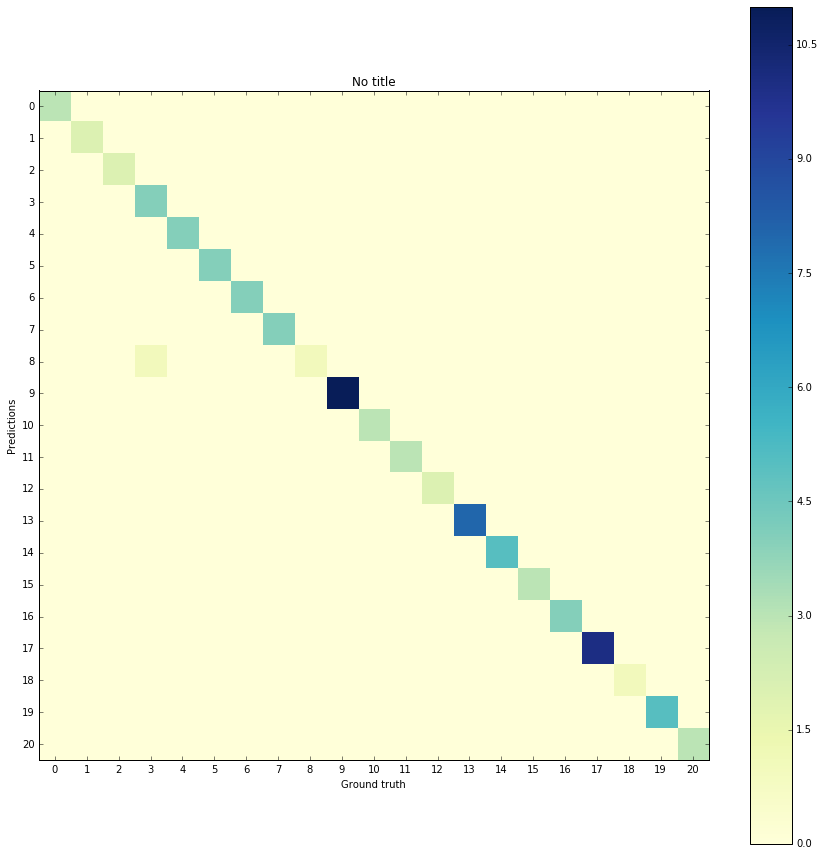
\includegraphics[width=0.4\textwidth]{classifier_svm_linear}
	\caption{Confusion matrix for linear SVM}
	\label{svm_linear}
\end{figure}
\end{multicols}

So the linear SVM has been chose, for its results better than the two other attempts. 

\subsection{Review on results}

The chosen classifier present only 0.5 accuracy. This middling performance is mainly due to the small size of the dataset. In order to improve the results several solution can be implemented.
\begin{itemize}
	\item Data processing: remove meaningless words (like "in", "my"...) change verbs by their infinitive form.
	\item Use of $n-gram$. This technique consist in using group of words to define a concept instead of words alone. First we look at one word, then 2 and 3 up to $n$.
\end{itemize}

\section{Interface}

\paragraph{}
We	have	the	opportunity	to	use	and	customize	the	telegram	chat	interface.	If	the	user	is	only	asked	to	make	a	selection	rather	than	enter	the	data,	the	options	can	be	presented	easily.	

\section{Questions logic}

\begin{figure}[H]
	\centering
	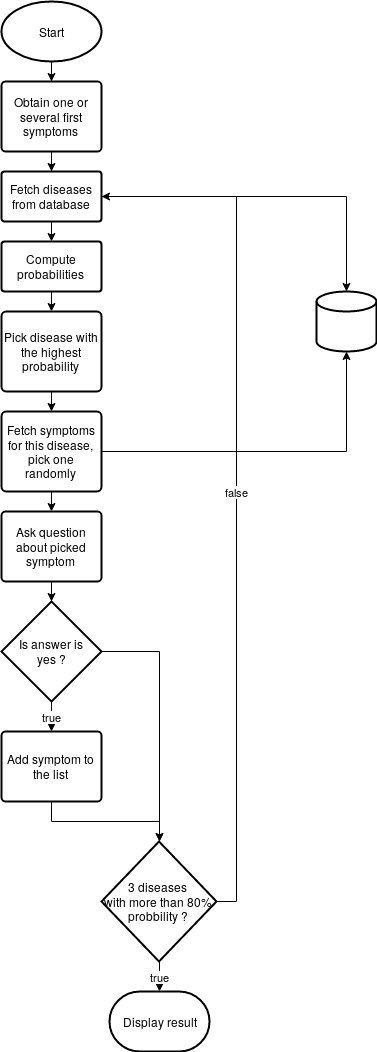
\includegraphics[height=0.9\textheight]{flow_chart_questions}
	\caption{Control flow graph showing the questions logic}
	\label{cfg_logic}
\end{figure}

\section{Decision making}

\paragraph{}
First,	we	get	personal	information	from	the	user	such	as	gender,	height,	weight,	etc.,	to	use	to	calculate	the	diagnosis	later.	We	then	take	the	user's	complaint	and	determine	which	of	the	symptoms	in	the	data	base	is	pointing	to.	We	find	diseases	with	this	symptom	by	searching	the	incoming	symptom	database.	Then,	we	ask	other	symptoms	of	these	diseases	whether	the	user	has	it.	If	the	patient	gives a	yes	response to	this	question,	we	increase the score	of the	diseases	that	the	symptom	belongs	to.	When	the	questions	are	over,	we	tell	the	patient	what	the	patients condition might be	and	we	give	advice	for	the	treatment.	We	then	aim	at	evaluating	personal	data	so	as	to	minimize	any	possible	equality	between	diseases	after	scoring.	In	this	project,	we	prepared	the	database	for	ourselves,	so	we	included	close	health	problems	similar	to	each	other	in	our	data	set.	At	this	point,	we	think	that	we	can	see	the	results	of	the	scoring	in	a	healthier	way.	